\documentclass[11pt,a4paper]{article}
\usepackage[T1]{fontenc}
\usepackage[utf8]{inputenc}
\usepackage{lmodern}
\usepackage[margin=25mm]{geometry}
\usepackage{amsmath,amssymb,amsthm,mathtools}
\usepackage{microtype}
\usepackage{booktabs}
\usepackage{graphicx}
\usepackage{xcolor}
\usepackage{hyperref}
\hypersetup{colorlinks=true,linkcolor=teal!55!black,citecolor=teal!55!black,
  urlcolor=violet!60!black,pdftitle={Sharp constants for sums of matrix moduli when 1<p<2},
  pdfauthor={Anonymous}}
\usepackage{enumitem}
\setlist{nosep,leftmargin=*}
\setlength{\emergencystretch}{2em}
\numberwithin{equation}{section}
\newtheorem{theorem}{Theorem}[section]
\newtheorem{lemma}[theorem]{Lemma}
\newtheorem{proposition}[theorem]{Proposition}
\newtheorem{corollary}[theorem]{Corollary}
\theoremstyle{definition}
\newtheorem{problem}[theorem]{Problem}
\theoremstyle{remark}
\newtheorem{remark}[theorem]{Remark}
\newtheorem{example}[theorem]{Example}
\DeclareMathOperator{\Tr}{Tr}
\DeclareMathOperator{\rank}{rank}
\DeclareMathOperator{\diag}{diag}
\DeclareMathOperator{\supp}{supp}
\newcommand{\C}{\mathbb C}
\newcommand{\R}{\mathbb R}
\newcommand{\norm}[1]{\left\lVert #1\right\rVert}
\newcommand{\abs}[1]{\left\lvert #1\right\rvert}
\newcommand{\ip}[2]{\left\langle #1,#2\right\rangle}

\title{Sharp constants for sums of matrix moduli when \(1<p<2\)\\[0.35em]
  \large The square case, an interpolation bound for Lee's problem,\\
  and certified failure of rank-one extremisers}
\author{Anonymous}
\date{Version 0.1.0-candidate, 15 November 2026. DOI \href{https://doi.org/10.5281/zenodo.24237738}{10.5281/zenodo.24237738}}

\begin{document}
\maketitle

\begin{abstract}
For complex matrices the modulus \(|A|=(A^*A)^{1/2}\) is not subadditive,
so one asks for the smallest constant \(c\) with
\(\|\sum_{k=1}^mA_k\|_p\le c\,\|\sum_{k=1}^m|A_k|\|_p\) in the Schatten
\(p\)-norm. This is Lee's problem for two summands and its
\(m\)-summand version due to Tang and Zhang. It is solved for
\(p\ge2\) (Qiu), but the conjectured formula fails for \(1<p<2\), where
the constants were listed as open as recently as October 2026. For
\(1<p<2\) and \(n\)-by-\(n\) matrices we prove three things. First,
when the number of summands is at least the dimension (\(m\ge n\)), the
best constant is an explicit one-variable maximum \(D_{p,n}\); it
depends only on the rank of \(\sum_k|A_k|\), every equality case is
classified, and for \(m<n\) the constant is strictly smaller. The
argument extends T.~Zhang's Frobenius-norm proof (\(p=2\)) to the whole
range \(1<p<2\), and the extremal family is Pang's, with its parameter
optimised. As a consequence the best constant for rank-one summands is
\(D_{p,\min(m,n)}\) in every dimension. Second, the best constant is
log-convex in \(1/p\); interpolating between \(p=1\) and \(p=2\) gives the
dimension-free bound \(((1+\sqrt m)/2)^{1-1/p}\), which improves the
previous bound \(m^{(p-1)/(2p)}\) for every \(m\ge2\). Third, for two
summands we certify, in exact rational and interval arithmetic, that
\(3\times3\) matrices beat the best rank-one value at nine exponents
between \(11/10\) and \(17/10\). So rank-one families do not solve
Lee's problem there. The exact dimension-free constants remain open.
\end{abstract}

\tableofcontents

\section{Introduction}\label{sec:intro}

This section explains the question, what was known, what this paper
adds and how it is organised.

\paragraph{The question.}
For complex numbers \(|a+b|\le|a|+|b|\). For a square matrix \(A\)
the natural modulus is \(|A|=(A^*A)^{1/2}\), the positive semidefinite
part of the polar decomposition \(A=U|A|\). This modulus is not
subadditive: in general \(|A+B|\not\le|A|+|B|\) in the positive
semidefinite order. Thompson \cite{Thompson} showed that subadditivity can be restored
up to unitary conjugations, \(|A+B|\le U|A|U^*+V|B|V^*\). A different
quantitative question asks how much larger the sum itself can be than
the sum of moduli, measured in a unitarily invariant norm. For the
Schatten \(p\)-norm \(\|X\|_p=(\Tr|X|^p)^{1/p}\) the answer quantifies how badly
the triangle inequality for matrix moduli can fail in the most commonly
used family of matrix norms. Precisely:

\begin{problem}[Lee; Tang--Zhang; T.~Zhang]\label{prob:main}
For \(1\le p\le\infty\) and integers \(m,n\ge1\), find the smallest
constant \(c_p(m,n)\) such that
\begin{equation}\label{eq:problem}
 \Bigl\|\sum_{k=1}^{m}A_k\Bigr\|_p\le c_p(m,n)
 \Bigl\|\sum_{k=1}^{m}|A_k|\Bigr\|_p
 \qquad\text{for all }A_1,\ldots,A_m\in M_n(\C),
\end{equation}
and the dimension-free constant \(c_p(m)=\sup_n c_p(m,n)\).
\end{problem}

Lee \cite{Lee2010,Lee2012} proved the bound \(\sqrt m\) for every
unitarily invariant norm and asked for the best Schatten constant when
\(m=2\); this is now called Lee's problem. Lee's conjectured Frobenius
value \(c_2(2)=\sqrt{(1+\sqrt2)/2}\) was proved by Lin and Zhang
\cite{LinZhang}. Tang and Zhang \cite{TangZhang} extended it to
\(c_2(m)=\sqrt{(1+\sqrt m)/2}\), proved
\(c_p(m)\le m^{(p-1)/(2p)}\) for all \(p\ge1\), and conjectured a closed
formula for \(c_p(m)\). T.~Zhang \cite{Zhang} introduced the
fixed-dimension constant \(c_p(m,n)\) (his Problem~1.14, written
\(c_p^{\mathrm{abs}}(m,n)\)), proved
\(c_2(m,n)=\sqrt{(1+\sqrt{\min(m,n)})/2}\) and
\(c_p(m,n)\le\min(m,n)^{(p-1)/(2p)}\). Qiu \cite{Qiu} proved the
Tang--Zhang formula for every \(p\ge2\). Below \(p=2\) the formula
fails: Zeng, Liu and Ratnavelu \cite{Zeng,ZengInterval}, Pang \cite{Pang}
and Qiu \cite{Qiu} gave counterexamples, all built from rank-one
matrices. The exact constants for \(1<p<2\) are listed as open by Qiu
\cite[Question 5.1]{Qiu}, by Li \cite[Problem 4.2]{Li}, and in the
October 2026 survey of Bourin and Zhang \cite[Problem 5.9]{BourinZhang}.
Table~\ref{tab:known} summarises the state of knowledge before this
paper.

\begin{table}[ht]
\centering
\small
\begin{tabular}{@{}lll@{}}
\toprule
\(p\) & dimension-free \(c_p(m)\) & fixed dimension \(c_p(m,n)\)\\
\midrule
\(1\) & \(1\) & \(1\)\\
\(1<p<2\) & open; \(\le m^{(p-1)/(2p)}\) \cite{TangZhang} &
  open; \(\le\min(m,n)^{(p-1)/(2p)}\) \cite{Zhang}\\
\(2\) & \(\sqrt{(1+\sqrt m)/2}\) \cite{LinZhang,TangZhang} &
  \(\sqrt{(1+\sqrt{\min(m,n)})/2}\) \cite{Zhang}\\
\(2<p<\infty\) & Tang--Zhang formula, proved by Qiu \cite{Qiu} & \\
\(\infty\) & \(\sqrt m\) \cite{TangZhang} & \(\sqrt{\min(m,n)}\) \cite{Zhang}\\
\bottomrule
\end{tabular}
\caption{What was known about Problem~\ref{prob:main} before this paper.
The exact two-rank-one value at \(p=3/2\) was found by Zeng, Liu and
Ratnavelu \cite{ZengExact}.}
\label{tab:known}
\end{table}

\paragraph{What is new.}
Throughout the paper \(1<p<2\). The results are stated precisely in
Section~\ref{sec:results}; in words they are as follows.
\begin{enumerate}
\item \emph{The square case.} When there are at least as many summands as
the dimension (\(m\ge n\)), the best constant is
\(c_p(m,n)=D_{p,n}\), an explicit one-variable maximum. More precisely
\(\|\sum A_k\|_p\le D_{p,r}\|\sum|A_k|\|_p\) with \(r\) the rank of
\(\sum|A_k|\). All equality cases are classified: every nonzero summand
has rank one and the summands form a weighted frame of a special shape.
For \(m<n\) the inequality \(c_p(m,n)<D_{p,n}\) is strict.
Consequently the best constant for rank-one summands is
\(D_{p,\min(m,n)}\) in every dimension, so for rank-one summands the
dimension-free problem is solved: the answer is \(D_{p,m}\).
\item \emph{An interpolation bound.} For fixed \(m,n\) the function
\(1/p\mapsto\log c_p(m,n)\) is convex. Interpolating between \(p=1\)
and \(p=2\) gives \(c_p(m)\le((1+\sqrt m)/2)^{1-1/p}\), which improves
the Tang--Zhang bound \(m^{(p-1)/(2p)}\) for every \(m\ge2\). Together
with item~1 this brackets the dimension-free constant within a factor
tending to \(2^{(2-p)/p}\) as \(m\to\infty\), instead of \(2^{1/p}\).
\item \emph{Rank one is not enough.} For two summands, explicit
\(3\times3\) matrices with exact rational entries beat the rank-one
value \(D_{p,2}\) at nine exponents \(p\) between \(11/10\) and
\(17/10\); this is certified by exact eigenvalue isolation and interval
arithmetic. Hence \(c_p(2)>D_{p,2}\) at these exponents, extending
Qiu's single numerical example at \(p=6/5\).
\end{enumerate}
The exact dimension-free constants \(c_p(m)\), including Lee's original
\(m=2\) case, remain open; Section~\ref{sec:open} lists what is left.

\paragraph{The idea, and what is borrowed.}
Write each \(A_k=U_k|A_k|\) and split \(|A_k|=|A_k|^{1/2}|A_k|^{1/2}\).
Then \(\sum A_k\) is a product of two block matrices, one controlled by
\(\Tr\sum|A_k|\) and the other by \(\sum|A_k|\) itself. For \(p=2\) this
is exactly T.~Zhang's proof \cite[Theorem 6.2]{Zhang}, with the Hölder
pair \((2,\infty)\). For \(1<p<2\) the right pair is \((2,2q)\) with
\[
 \frac1p=\frac12+\frac1{2q},\qquad q=\frac{p}{2-p}.
\]
The bound then depends only on the eigenvalues of \(\sum|A_k|\), and
maximising it over the eigenvalues is a question about two power sums
(equivalently two Rényi entropies) on the probability simplex. Its
answer, one large eigenvalue and the rest equal, is a special case of
known results of Harremoës \cite{Harremoes} and Sakai and Iwata
\cite{SakaiIwata}; we give a short self-contained proof together with
the uniqueness of the optimal ratio, which we need for the equality
cases. For \(p=3/2\) and rank-one summands the same factorisation is
Lemma~3.1 of Zeng, Liu and Ratnavelu \cite{ZengExact}. The matching
lower bound uses the two-equiangular-system family of Pang \cite{Pang}
with its free parameter re-optimised. What is new here is the matching
upper bound for every \(1<p<2\) and every dimension, its exact range
\(m\ge n\), the classification of equality cases, the interpolation
bound, and the certified rank-one failure.

\paragraph{Roadmap.}
Section~\ref{sec:results} fixes notation and states all results.
Section~\ref{sec:scalar} solves the scalar problem on the simplex.
Section~\ref{sec:upper} proves the upper bound and its sharpness.
Section~\ref{sec:equality} classifies equality and proves strictness
for \(m<n\). Section~\ref{sec:values} gives explicit values and
asymptotics. Section~\ref{sec:interp} proves the interpolation theorem
and the dimension-free bound. Section~\ref{sec:beyond} presents the
certified witnesses beyond rank one. Section~\ref{sec:concave} records
a consequence for concave functions via Li's transfer theorem, and
Section~\ref{sec:open} lists open problems.

\section{Notation and main results}\label{sec:results}

This section fixes notation and states every result of the paper;
proofs follow in later sections.

\paragraph{Notation.}
\(M_n(\C)\) is the space of complex \(n\times n\) matrices;
\(|A|=(A^*A)^{1/2}\) and \(\|A\|_p=(\Tr|A|^p)^{1/p}\), also for
rectangular matrices, with \(\|A\|_\infty\) the operator norm. Inner
products \(\ip{x}{y}=y^*x\) are linear in the first slot. For a
positive semidefinite \(B\), powers \(B^s\) with \(s\le0\) or complex
\(s\) are taken on the support \(\supp B=\operatorname{ran}B\) and set
to zero on its orthogonal complement. We fix
\begin{equation}\label{eq:q}
 1<p<2,\qquad q=\frac{p}{2-p}\in(p,\infty),
 \qquad\text{so that}\qquad \frac1p=\frac12+\frac1{2q}.
\end{equation}
The probability simplex is
\(\Delta_d=\{\lambda\in[0,1]^d:\sum_i\lambda_i=1\}\), and
\(S_s(\lambda)=\sum_i\lambda_i^s\).

\paragraph{The constant \(D_{p,d}\).}
For \(d\ge2\) put \(a=d-1\) and
\begin{equation}\label{eq:F}
 F_{p,d}(x)=
 \frac{\sqrt{x+a}\,(x^q+a)^{1/(2q)}}{(x^p+a)^{1/p}},
 \qquad x\ge1.
\end{equation}
In words, \(F_{p,d}(x)\) is the quotient
\(S_1^{1/2}S_q^{1/(2q)}/S_p^{1/p}\) evaluated at the probability vector
\((x,1,\ldots,1)/(x+d-1)\), which has one coordinate \(x\) times
larger than the other \(d-1\) equal coordinates. Lemma~\ref{lem:scalar}
shows that \(F_{p,d}\) has a unique maximiser \(x_{p,d}>1\), the unique
solution \(x>1\) of
\begin{equation}\label{eq:critical}
 \frac{1}{x+a}+\frac{x^{q-1}}{x^q+a}-\frac{2x^{p-1}}{x^p+a}=0.
\end{equation}
Set \(D_{p,d}=F_{p,d}(x_{p,d})\) for \(d\ge2\) and \(D_{p,1}=1\). At the endpoints we put
\(D_{1,d}=1\) and \(D_{2,d}=\sqrt{(1+\sqrt d)/2}\), the limits of \(D_{p,d}\) as
\(p\downarrow1\) and \(p\uparrow2\) (Proposition~\ref{prop:asymptotic}). For
example \(D_{3/2,2}=1.0364143573\ldots\) and \(D_{6/5,2}=1.0073249657\ldots\).

\subsection{The square case}

\begin{theorem}[Sharp dimension bound]\label{thm:main}
Let \(A_1,\ldots,A_m\in M_n(\C)\) with \(B=\sum_k|A_k|\ne0\), and let
\(r=\rank B\). Then
\begin{equation}\label{eq:main}
 \Bigl\|\sum_{k=1}^{m}A_k\Bigr\|_p
 \le D_{p,r}\|B\|_p\le D_{p,n}\|B\|_p .
\end{equation}
For every \(m\ge n\), \(c_p(m,n)=D_{p,n}\). For \(1\le m<n\),
\(c_p(m,n)<D_{p,n}\). The equality cases are classified in
Theorem~\ref{thm:equality}: every nonzero summand of an extremal family
has rank one.
\end{theorem}

\begin{corollary}[Rank-one summands]\label{cor:rankone}
If \(\rank A_k\le1\) for every \(k\) and \(d=\min(m,n)\), then
\begin{equation}\label{eq:rankone}
 \Bigl\|\sum_{k=1}^{m}A_k\Bigr\|_p
 \le D_{p,d}\Bigl\|\sum_{k=1}^{m}|A_k|\Bigr\|_p,
\end{equation}
and the constant is optimal for every \(m,n\). In particular the
dimension-free best constant for \(m\) rank-one summands is \(D_{p,m}\).
\end{corollary}

Compared with T.~Zhang's bound \(\min(m,n)^{(p-1)/(2p)}\), the exact
value \(D_{p,n}\) is smaller by a factor tending to \(2^{-1/p}\)
(Proposition~\ref{prop:asymptotic}); for example
\(D_{3/2,10}=1.16995\ldots\) against \(10^{1/6}=1.46780\ldots\).
For \(m<n\), however, \(D_{p,n}\) can be a weaker bound than the known
\(m\)-dependent ones; Corollary~\ref{cor:interp} gives the best bound
we know there.

\subsection{Interpolation in the exponent}

\begin{theorem}[Log-convexity]\label{thm:interp}
Fix \(m,n\ge1\). For \(1\le p_0<p_1\le\infty\), \(0<\theta<1\) and
\(1/p_\theta=(1-\theta)/p_0+\theta/p_1\),
\[
 c_{p_\theta}(m,n)\le c_{p_0}(m,n)^{1-\theta}\,c_{p_1}(m,n)^{\theta}.
\]
The same holds for the dimension-free constants \(c_p(m)\).
\end{theorem}

\begin{corollary}[Dimension-free bound]\label{cor:interp}
For \(1\le p\le2\) and all \(m,n\ge1\),
\begin{equation}\label{eq:interpbound}
 c_p(m,n)\le\Bigl(\frac{1+\sqrt{\min(m,n)}}{2}\Bigr)^{1-1/p},
 \qquad
 D_{p,m}\le c_p(m)\le\Bigl(\frac{1+\sqrt m}{2}\Bigr)^{1-1/p}.
\end{equation}
For every \(m\ge2\) and \(1<p<2\) the upper bound is strictly smaller
than the Tang--Zhang bound \(m^{(p-1)/(2p)}\), and the ratio of the upper
to the lower bound in \eqref{eq:interpbound} tends to \(2^{(2-p)/p}\)
as \(m\to\infty\) (against \(2^{1/p}\) for the Tang--Zhang bound).
For \(m<n\), \(c_p(m,n)\le\min\{D_{p,n},((1+\sqrt m)/2)^{1-1/p}\}\).
\end{corollary}

For Lee's original problem (\(m=2\)) at \(p=3/2\), for example, this
gives \(1.03641\le c_{3/2}(2)\le1.06476\) (Proposition~\ref{prop:certified} below raises the lower bound to \(1.036425\)), where the previous upper
bound was \(2^{1/6}=1.12247\ldots\) (Table~\ref{tab:bounds} and
Figure~\ref{fig:bounds} in Section~\ref{sec:interp}).

\subsection{Beyond rank one}

\begin{proposition}[Certified failure of rank-one extremisers]
\label{prop:certified}
For each
\[
 p\in\Bigl\{\tfrac{11}{10},\tfrac65,\tfrac54,\tfrac{13}{10},\tfrac43,
 \tfrac75,\tfrac32,\tfrac85,\tfrac{17}{10}\Bigr\}
\]
there are real \(3\times3\) matrices \(A_1,A_2\) with rational entries
and
\[
 \frac{\|A_1+A_2\|_p}{\||A_1|+|A_2|\|_p}>D_{p,2}.
\]
Consequently \(c_p(2,n)>c_p(2,2)=D_{p,2}\) for every \(n\ge3\), and
\(c_p(2)>D_{p,2}\), at each of these exponents.
\end{proposition}

At \(p=6/5\) a numerical example of this kind was given by Qiu
\cite[Section 5]{Qiu}. Two remarks put the proposition in context. At
\(p=2\) there is no such gap: \(c_2(2,n)=c_2(2,2)\) for every \(n\ge2\)
\cite[Theorem 6.2]{Zhang}. Numerically the gap shrinks quickly as \(p\)
approaches \(2\) (Section~\ref{sec:beyond}).

\section{The scalar extremum}\label{sec:scalar}

This section solves the optimisation problem on the simplex to which the
matrix inequality will be reduced in Section~\ref{sec:upper}.

\begin{lemma}\label{lem:scalar}
For \(d\ge2\),
\begin{equation}\label{eq:simplex}
 \max_{\lambda\in\Delta_d}\Phi(\lambda)=D_{p,d},
 \qquad
 \Phi(\lambda)=\frac{S_q(\lambda)^{1/(2q)}}{S_p(\lambda)^{1/p}}.
\end{equation}
Every maximiser is a permutation of
\begin{equation}\label{eq:spectrum}
 \frac{(x_{p,d},1,\ldots,1)}{x_{p,d}+d-1}.
\end{equation}
Moreover \(D_{p,d+1}>D_{p,d}\) for every \(d\ge1\), and
\eqref{eq:critical} has exactly one solution \(x>1\).
\end{lemma}

Note that on \(\Delta_d\) we have \(S_1=1\), so \(\Phi\) equals the
quotient \(S_1^{1/2}S_q^{1/(2q)}/S_p^{1/p}\) that defines \(F_{p,d}\).

\begin{proof}
\(\Phi\) is continuous and positive on the compact set \(\Delta_d\), so
a maximiser exists. Write \(f=\log\Phi\).

\emph{Step 1: full support.} Suppose \(\lambda\in\Delta_d\) has a zero
coordinate. Multiply its coordinates by \(1-\varepsilon\) and place
\(\varepsilon\) in one zero coordinate. For \(s>1\) the new power sum is
\((1-\varepsilon)^sS_s+\varepsilon^s=(1-\varepsilon)^sS_s\,(1+o(\varepsilon))\), because
\(\varepsilon^s=o(\varepsilon)\). Hence
\[
 f(\lambda(\varepsilon))-f(\lambda)
 =\frac{1}{2q}\log(1-\varepsilon)^q-\frac1p\log(1-\varepsilon)^p+o(\varepsilon)
 =-\frac12\log(1-\varepsilon)+o(\varepsilon)=\frac{\varepsilon}{2}+o(\varepsilon)>0
\]
for small \(\varepsilon>0\). Hence no boundary point is a
maximiser. Applying the same perturbation to a maximiser in
\(\Delta_d\), viewed inside \(\Delta_{d+1}\), gives
\(D_{p,d+1}>D_{p,d}\) (also for \(d=1\), where \(D_{p,1}=1\)).

\emph{Step 2: two levels.} At an interior critical point of \(f\) on
\(\{\sum_i\lambda_i=1\}\) there is a multiplier \(\mu\) with
\[
 \frac{\lambda_i^{q-1}}{2S_q}-\frac{\lambda_i^{p-1}}{S_p}=\mu
 \qquad(1\le i\le d).
\]
Multiplying by \(\lambda_i\) and summing gives \(\mu=\frac12-1=-\frac12\).
So every coordinate is a positive root of
\begin{equation}\label{eq:h}
 h(t)=\frac{t^{q-1}}{S_q}-\frac{2t^{p-1}}{S_p}+1,
 \qquad
 h'(t)=t^{p-2}\Bigl(\frac{q-1}{S_q}t^{q-p}-\frac{2(p-1)}{S_p}\Bigr).
\end{equation}
The bracket in \(h'\) increases strictly in \(t\), so \(h'\) changes
sign once, from negative to positive; hence \(h\) is decreasing and then
increasing, and has at most two positive roots. At the uniform vector,
for \(z\) with \(\sum_iz_i=0\), the second variation of \(f\) is
\[
 d\Bigl(\frac{q-1}{2}-(p-1)\Bigr)\sum_iz_i^2
 =\frac{d(p-1)^2}{2-p}\sum_iz_i^2>0,
\]
so the uniform vector is a strict local minimum of \(f\), and hence not
a global maximiser. Therefore a maximiser takes exactly two distinct
values \(b<c\). The two roots of \(h\) lie on either side of the unique
minimum of \(h\), so \(h'(c)>0\).

\emph{Step 3: the large value occurs once.} Suppose two coordinates
\(i\ne j\) equal \(c\), and move along \(z=e_i-e_j\). Because
\(\lambda_i=\lambda_j\), the first variations of \(S_q\) and \(S_p\)
along \(z\) vanish, and the second variation of \(f\) is
\[
 \frac{(q-1)c^{q-2}}{S_q}-\frac{2(p-1)c^{p-2}}{S_p}=h'(c)>0,
\]
contradicting maximality. Hence exactly one coordinate equals \(c\).
Writing \(x=c/b>1\) gives a vector of the form \eqref{eq:spectrum}, and
\(\Phi\) of that vector is \(F_{p,d}(x)\) by \eqref{eq:F}.

\emph{Step 4: uniqueness of the parameter.} Since
\(\frac{d}{dx}\log F_{p,d}\) is one half of the left side of
\eqref{eq:critical}, critical points of \(F_{p,d}\) on \((1,\infty)\)
are solutions of \eqref{eq:critical}. Put \(r=p-1\in(0,1)\) and
\(x=\exp(\frac{1-r}{r}z)\) with \(z>0\). Clearing the positive
denominators in \eqref{eq:critical} gives
\begin{equation}\label{eq:hyperbolic}
 a=\exp\bigl((r^{-1}-r)z\bigr)\,
   \frac{\cosh z-\exp(rz)}{\cosh z-\exp(-rz)} .
\end{equation}
The denominator is positive for \(z>0\). There is a unique \(z_0>0\) with
\(\cosh z_0=\exp(rz_0)\): indeed \(\log(\cosh z)/z\) increases strictly
from \(0\) to \(1\), since its derivative has the sign of
\(z\tanh z-\log\cosh z\), whose derivative is \(z\operatorname{sech}^2z>0\).
The right side of \eqref{eq:hyperbolic} is negative on \((0,z_0)\). On
\((z_0,\infty)\) its quotient factor is positive and strictly increasing,
because the derivative of the quotient has the sign of
\[
 N(z)=\sinh z\sinh(rz)-r\cosh z\cosh(rz)+r,
 \qquad N(0)=0,\qquad N'(z)=(1-r^2)\cosh z\sinh(rz)>0.
\]
The exponential factor also increases strictly, so the right side
increases from \(0\) to \(\infty\) on \((z_0,\infty)\) and equals \(a>0\)
exactly once. So \eqref{eq:critical} has exactly one solution \(x>1\).

\emph{Step 5: conclusion.} By Steps 1--3, a global maximiser of \(\Phi\)
has the form \eqref{eq:spectrum} for some \(x^*>1\). Since every
\(F_{p,d}(x)\) is a value of \(\Phi\), \(x^*\) maximises \(F_{p,d}\) on
\((1,\infty)\), so it is a critical point, and by Step~4 it is
\(x_{p,d}\). Hence the maximum is \(D_{p,d}\) and every maximiser is a
permutation of \eqref{eq:spectrum}.
\end{proof}

\begin{remark}[Entropy form and prior work]\label{rem:entropy}
For \(s>1\) let \(H_s(\lambda)=(1-s)^{-1}\log S_s(\lambda)\) be the
Rényi entropy. Since \((q-1)/(2q)=(p-1)/p\),
\begin{equation}\label{eq:entropy}
 \log D_{p,d}=\frac{p-1}{p}\max_{\lambda\in\Delta_d}
 \bigl(H_p(\lambda)-H_q(\lambda)\bigr).
\end{equation}
The one-large, rest-equal shape of the maximiser is a special case of the
joint range of two Rényi entropies (Harremoës \cite[Theorem 3]{Harremoes})
and of sharp bounds between \(\ell^p\) and \(\ell^q\) norms on the
simplex (Sakai and Iwata \cite[Theorem 1]{SakaiIwata}, family \(v_n\)).
Steps 1--3 are included to keep the paper self-contained; Step~4, the
uniqueness for the linked exponents \(q=p/(2-p)\), is used in the
equality analysis.
\end{remark}

\section{The upper bound and its sharpness}\label{sec:upper}

This section proves inequality \eqref{eq:main} by a Hölder
factorisation, extending T.~Zhang's \(p=2\) argument, and shows that it
is attained by Pang's family.

\paragraph{Factorisation.}
Let \(A_k=U_kH_k\) be polar decompositions with \(H_k=|A_k|\) and
\(U_k\) unitary. Form the \(n\times mn\) block rows
\[
 X=\bigl[U_1H_1^{1/2}\ \cdots\ U_mH_m^{1/2}\bigr],
 \qquad
 Y=\bigl[H_1^{1/2}\ \cdots\ H_m^{1/2}\bigr].
\]
Then \(XY^*=\sum_kA_k\), \(YY^*=\sum_kH_k=B\) and
\(\|X\|_2^2=\Tr XX^*=\sum_k\Tr H_k=\Tr B\). Since \(1/p=1/2+1/(2q)\),
the Schatten Hölder inequality gives
\begin{equation}\label{eq:factor}
 \Bigl\|\sum_kA_k\Bigr\|_p\le\|X\|_2\,\|Y^*\|_{2q}
 =(\Tr B)^{1/2}(\Tr B^q)^{1/(2q)}.
\end{equation}
At \(p=2\) (so \(q=\infty\)) this is the first step of T.~Zhang's proof
of \(c_2(m,n)=\sqrt{(1+\sqrt{\min(m,n)})/2}\) \cite[Theorem 6.2]{Zhang};
at \(p=3/2\) and for rank-one summands it is Lemma~3.1 of Zeng, Liu and
Ratnavelu \cite{ZengExact}.

\begin{proof}[Proof of the upper bound in Theorem~\ref{thm:main}]
Divide \eqref{eq:factor} by \(\|B\|_p\). The right side is homogeneous
of degree zero in \(B\), so we may normalise the nonzero eigenvalues of
\(B\) to a vector \(\lambda\in\Delta_r\), \(r=\rank B\). The quotient
becomes \(\Phi(\lambda)\le D_{p,r}\) by Lemma~\ref{lem:scalar} (for
\(r=1\) it equals \(1=D_{p,1}\)). Since \(D_{p,d}\) increases with \(d\)
and \(r\le n\), \eqref{eq:main} follows. If every \(A_k\) has rank at
most one then \(r\le\min(m,n)\), which proves \eqref{eq:rankone}.
\end{proof}

\begin{remark}[Splitting into rank-one terms]\label{rem:splitting}
If \(A=\sum_js_ju_jv_j^*\) is a singular value decomposition, then
\(|s_ju_jv_j^*|=s_jv_jv_j^*\) and \(\sum_js_jv_jv_j^*=|A|\). So replacing
each \(A_k\) by its rank-one singular terms preserves both \(\sum_kA_k\)
and \(\sum_k|A_k|\) (while increasing the number of summands). This is why
the rank-one bound of \cite[Lemma 3.1]{ZengExact} already implies
\eqref{eq:factor} at \(p=3/2\) for arbitrary matrices. It also shows that
the \(m\ge n\) part of Theorem~\ref{thm:main} cannot be obtained by
counting summands: what matters is the rank of \(B\).
\end{remark}

\paragraph{Sharpness: Pang's two-Gram family.}
Fix \(d\ge2\), write \(x=x_{p,d}\), and set
\[
 s=\frac{x-1}{x+d-1},\qquad t=\frac{x^q-1}{x^q+d-1}.
\]
Let \(J_d\) be the all-ones matrix and
\begin{equation}\label{eq:twoGram}
 G=(1-s)I_d+sJ_d,\qquad L=(1-t)I_d+tJ_d .
\end{equation}
Both are positive definite with unit diagonal, so they are Gram matrices
of unit vectors \(v_1,\ldots,v_d\) and \(u_1,\ldots,u_d\) in \(\R^d\);
these are \emph{equiangular} systems, in which all pairwise inner products
are equal (to \(s\) and \(t\) respectively). This is the family used by
Pang \cite{Pang}, where the parameter was fixed by the Tang--Zhang
equation; here it is chosen to maximise \eqref{eq:F}. Its \(p=2\) limit
(\(q=\infty\), \(t=1\), a single common left vector) is the sharpness
family in Step~3 of T.~Zhang's proof \cite[Theorem 6.2]{Zhang}, and for
\(d=2\) the family is among the real two-vector configurations of Qiu
\cite[Section 5]{Qiu}, whose numerical maximum agrees with \(D_{p,2}\). Put
\(A_k=u_kv_k^*\). If \(U,V\) have columns \(u_k,v_k\), then
\(\sum_kA_k=UV^*\) and \(\sum_k|A_k|=\sum_kv_kv_k^*=VV^*\), whose nonzero
eigenvalues are those of \(G=V^*V\):
\[
 \frac{dx}{x+d-1}\quad\text{and}\quad
 \frac{d}{x+d-1}\ \ (\text{multiplicity }d-1).
\]
The eigenvalues of \(L\) have the same form with \(x\) replaced by
\(x^q\). The squared singular values of \(UV^*\) are the eigenvalues of
\(VU^*UV^*\), that is of \(G^{1/2}LG^{1/2}\), and since \(G\) and \(L\)
commute these are the eigenvalues of \(LG\). Using \(p(q+1)/2=q\), a
direct substitution gives
\begin{equation}\label{eq:sharpconstruction}
 \frac{\|\sum_{k=1}^{d}A_k\|_p}{\|\sum_{k=1}^{d}|A_k|\|_p}
 =F_{p,d}(x_{p,d})=D_{p,d}.
\end{equation}
For \(m\ge n\) take \(d=n\) and append zero matrices (or split one
summand into positive multiples, so that every summand is nonzero). For
the rank-one problem take \(d=\min(m,n)\) and embed the construction in
\(\C^n\). This proves \(c_p(m,n)=D_{p,n}\) for \(m\ge n\) and the
optimality in Corollary~\ref{cor:rankone}; since a rank-one family of
\(m\) summands in any dimension has \(\rank B\le m\), the dimension-free
rank-one constant is \(D_{p,m}\).

\section{Equality cases and strictness}\label{sec:equality}

This section identifies exactly which families attain the bound and uses
this to prove that the bound is strict when \(m<n\). The key tool is the
equality case of Hölder's inequality in a rectangular form, needed
because the ambient dimension may exceed the rank of \(B\).

\begin{lemma}[Rectangular equality condition]\label{lem:holder}
Let \(Y\in\C^{d\times N}\) with \(YY^*=B>0\), and let
\(0\ne X\in\C^{e\times N}\) with \(e\ge d\). Then
\begin{equation}\label{eq:rectholder}
 \|XY^*\|_p\le\|X\|_2(\Tr B^q)^{1/(2q)},
\end{equation}
with equality if and only if
\begin{equation}\label{eq:recteq}
 X=\gamma\,WB^{(q-1)/2}Y
\end{equation}
for some \(\gamma>0\) and an isometry \(W:\C^d\to\C^e\) (a unitary if
\(e=d\)).
\end{lemma}

\begin{proof}
Let \(p'=p/(p-1)>2\); then \(q\) is the conjugate exponent of \(p'/2\).
Choose \(Z\in\C^{e\times d}\) with \(\|Z\|_{p'}=1\) and
\(\|XY^*\|_p=\abs{\Tr(ZY)^*X}\) (Schatten duality). For this \(Z\),
Hilbert--Schmidt Cauchy--Schwarz and trace Hölder give
\[
 \|XY^*\|_p=\abs{\Tr(ZY)^*X}\le\|X\|_2\,\|ZY\|_2
 =\|X\|_2(\Tr Z^*ZB)^{1/2}
 \le\|X\|_2\,\|Z^*Z\|_{p'/2}^{1/2}\,(\Tr B^q)^{1/(2q)},
\]
and \(\|Z^*Z\|_{p'/2}=\|Z\|_{p'}^2=1\). This proves \eqref{eq:rectholder},
and equality holds if and only if both inequalities are equalities for
this same \(Z\).

\emph{Equality in trace Hölder.} We claim that, for \(T\ge0\) with
\(\|T\|_{p'/2}=1\), \(\Tr TB=(\Tr B^q)^{1/q}\) forces
\(T=cB^{q-1}\) with \(c>0\). Let \(\mathcal E(T)\) be the pinching of
\(T\) to the eigenspaces of \(B\). Then \(\Tr\mathcal E(T)B=\Tr TB>0\) and
\(\|\mathcal E(T)\|_{p'/2}\le\|T\|_{p'/2}\), with strict inequality
unless \(\mathcal E(T)=T\), because \(1<p'/2<\infty\) and the
\(p'/2\)-norm is strictly convex. If the inequality were strict, then
\(\mathcal E(T)/\|\mathcal E(T)\|_{p'/2}\) would have norm one and a
strictly larger value of \(\Tr(\cdot)B\), contradicting the maximality of
\(T\) (trace Hölder says \((\Tr B^q)^{1/q}\) is the maximum). So \(T\)
commutes with \(B\). In a common eigenbasis, with eigenvalues \(t_i\) of
\(T\) and \(b_i\) of \(B\), scalar Hölder equality gives
\(t_i^{p'/2}\propto b_i^q\), that is \(t_i\propto b_i^{q-1}\), because
\((p'/2-1)^{-1}=q-1\). Hence \(Z^*Z=cB^{q-1}\), which is invertible, so
\(Z=W(cB^{q-1})^{1/2}\) with \(W\) an isometry (the polar factor of \(Z\)).

\emph{Equality in Cauchy--Schwarz} means \(X=\gamma' ZY\) for a scalar
\(\gamma'\); absorbing its phase into \(W\) gives \eqref{eq:recteq}.
Conversely, substituting \eqref{eq:recteq} and using \(p(q+1)/2=q\)
gives equality in \eqref{eq:rectholder}.
\end{proof}

\begin{theorem}[All equality cases]\label{thm:equality}
Let \(n\ge2\) and let \(A_1,\ldots,A_m\in M_n(\C)\) be not all zero.
Scale them so that \(\Tr B=1\), where \(B=\sum_k|A_k|\). Put
\(x=x_{p,n}\),
\[
 \alpha=\frac{x}{x+n-1},\qquad\beta=\frac{1}{x+n-1}.
\]
Equality holds in \eqref{eq:main} with constant \(D_{p,n}\) if and only if
there are a unit vector \(w\), a unitary \(W\), and, for the nonzero
summands, weights \(r_k>0\) and unit vectors \(v_k\) such that
\begin{align}
 B&=\alpha ww^*+\beta(I-ww^*),\label{eq:Bequality}\\
 \sum_kr_kv_kv_k^*&=B,\qquad \abs{\ip{w}{v_k}}^2=\alpha,\label{eq:frame}\\
 A_k&=\frac{r_k}{\sqrt{S_q}}\,WB^{(q-1)/2}v_kv_k^*,
 \qquad S_q=\Tr B^q.\label{eq:Aequality}
\end{align}
Taking traces in \eqref{eq:frame} shows \(\sum_kr_k=\Tr B=1\). Zero
summands may be added freely. Every nonzero summand has rank one, so at
least \(n\) summands are nonzero.
\end{theorem}

In words: an extremal family is a weighted frame \((r_k,v_k)\) whose frame
operator has one large and \(n-1\) equal small eigenvalues, all of whose
vectors make the same angle with the large eigendirection \(w\), and the
left factors are then forced by \eqref{eq:Aequality}.

\begin{proof}
Equality with constant \(D_{p,n}\) forces \(\rank B=n\), because
\(D_{p,r}<D_{p,n}\) for \(r<n\) (Lemma~\ref{lem:scalar}); it then forces
equality both in the scalar bound and in \eqref{eq:factor}.
Lemma~\ref{lem:scalar} gives \eqref{eq:Bequality}
(in particular \(B>0\)), and Lemma~\ref{lem:holder} with \(e=d=n\) and
\(\|X\|_2^2=\Tr B=1\) gives
\(X=S_q^{-1/2}WB^{(q-1)/2}Y\). Comparing the \(k\)-th blocks,
\(U_kH_k^{1/2}=S_q^{-1/2}WB^{(q-1)/2}H_k^{1/2}\); multiplying each side by
its adjoint on the left and using that \(U_k,W\) are unitary yields
\begin{equation}\label{eq:neutral}
 H_k^{1/2}\bigl(B^{q-1}-S_qI\bigr)H_k^{1/2}=0 .
\end{equation}
The Hermitian matrix \(T=B^{q-1}-S_qI\) has one positive and \(n-1\)
negative eigenvalues, because
\(S_q=\alpha\cdot\alpha^{q-1}+(1-\alpha)\beta^{q-1}\) lies strictly
between \(\beta^{q-1}\) and \(\alpha^{q-1}\); \(T\) is negative definite on
\(w^\perp\). By \eqref{eq:neutral}, the range of \(H_k^{1/2}\) is totally
isotropic for \(T\). A subspace of dimension at least two meets
\(w^\perp\) nontrivially, where \(T\) is strictly negative, so it cannot be
totally isotropic. Hence \(\rank H_k\le1\).

Write each nonzero \(H_k=r_kv_kv_k^*\). Then \eqref{eq:neutral} reads
\(\ip{B^{q-1}v_k}{v_k}=S_q\). With \(c_k=\abs{\ip{w}{v_k}}^2\) the left
side is \(\alpha^{q-1}c_k+\beta^{q-1}(1-c_k)\), while
\(S_q=\alpha^q+(n-1)\beta^q=\alpha^{q-1}\alpha+\beta^{q-1}(1-\alpha)\)
(using \(\alpha+(n-1)\beta=1\)). Since \(\alpha^{q-1}\ne\beta^{q-1}\), the
condition is exactly \(c_k=\alpha\), which is \eqref{eq:frame}. The block
equality gives \eqref{eq:Aequality}. This proves necessity.

Conversely, \eqref{eq:frame} gives \(\|B^{(q-1)/2}v_k\|^2=S_q\), so
\(|A_k|=r_kv_kv_k^*\), \(\sum_k|A_k|=B\), and
\(\sum_kA_k=S_q^{-1/2}WB^{(q-1)/2}\sum_kr_kv_kv_k^*=S_q^{-1/2}WB^{(q+1)/2}\).
Its \(p\)-norm divided by \(\|B\|_p\) equals \(\Phi\) of the spectrum of
\(B\), which is \(D_{p,n}\). Finally \(\rank B=n\) and
\(B=\sum_kr_kv_kv_k^*\) require at least \(n\) nonzero summands.
\end{proof}

\begin{proof}[Proof of strictness in Theorem~\ref{thm:main}]
Let \(m<n\). Normalise \(\sum_k\|A_k\|_1=1\). The set of such families is
compact, and on it \(\|B\|_p\ge n^{1/p-1}\|B\|_1=n^{1/p-1}>0\) (as
\(\Tr B=\sum_k\|A_k\|_1\)). So the quotient is continuous there and the
supremum \(c_p(m,n)\) is attained. If it equalled \(D_{p,n}\),
Theorem~\ref{thm:equality} would require at least \(n>m\) nonzero
summands, which is impossible.
\end{proof}

\begin{corollary}[Equality for rank-one summands, \(n\ge m\)]
\label{cor:rankoneequality}
Let \(n\ge m\ge2\), let \(\rank A_k\le1\) for all \(k\), and suppose the
\(A_k\) are not all zero. Equality holds in \eqref{eq:rankone} if and only
if, up to common left and right unitary transformations, a common positive
scale and phases in the rank-one factorisations,
\(A_k=\rho\,u_kv_k^*\) with \(\rho>0\) and unit vectors whose Gram matrices
are \(L\) and \(G\) of \eqref{eq:twoGram} with \(d=m\), \(x=x_{p,m}\).
\end{corollary}

\begin{proof}
Since \(D_{p,d}\) increases strictly in \(d\), equality forces
\(\rank B=m\); in particular every summand is nonzero. Let
\(E:\C^m\to\C^n\) be an isometry onto \(\supp B\), \(B_0=E^*BE>0\), and
replace \(Y\) by \(Y_0=E^*Y\) (allowed because the columns of \(Y\) lie in
\(\supp B\)). Then \(Y_0Y_0^*=B_0\) and \(XY^*=(XY_0^*)E^*\), and right
multiplication by \(E^*\) preserves singular values. So
Lemma~\ref{lem:holder} applies with \(d=m\), \(e=n\), and an isometry
\(W:\C^m\to\C^n\). Repeating the proof of Theorem~\ref{thm:equality}
inside \(\supp B\), with \(B^{q-1}\) read as \(EB_0^{q-1}E^*\) and \(I\) as
the support projection, gives the same spectral form
\eqref{eq:Bequality} for \(B_0\) and the fixed-angle condition
\eqref{eq:frame}.

Normalise \(\Tr B=1\) and let \(Z\) be the \(m\times m\) matrix (in
\(\supp B\)) with columns \(\sqrt{r_k}v_k\). Its Gram matrix \(G_0=Z^*Z\)
has the eigenvalues \(\alpha,\beta,\ldots,\beta\) of \(B_0=ZZ^*\). The
vector \(z=Z^*w/\sqrt\alpha\) is a unit eigenvector of \(G_0\) for
\(\alpha\), and \(|z_k|^2=r_k\abs{\ip{w}{v_k}}^2/\alpha=r_k\). Since
\((G_0)_{kk}=r_k\),
\(r_k=\beta+(\alpha-\beta)|z_k|^2=\beta+(\alpha-\beta)r_k\), and with
\(\alpha+(m-1)\beta=1\) this forces \(r_k=1/m\). Adjusting phases makes
\(z\) the flat unit vector, so the Gram matrix of the \(v_k\) is
\(mG_0=G\). The isometry \(W\) preserves inner products, so by
\eqref{eq:Aequality} the unit left vectors have Gram matrix
\((m/S_q)G_0^q=L\). This proves necessity; Section~\ref{sec:upper} proves
sufficiency.
\end{proof}

\begin{remark}[More summands than dimensions]\label{rem:harmonic}
For \(m>n\) Theorem~\ref{thm:equality} allows extremal frames that are
not splittings of an \(n\)-summand extremiser. For example, with
\(\zeta=e^{2\pi i/m}\), \(r_k=1/m\) and
\(v_k=(\sqrt\alpha,\sqrt\beta\,\zeta^k,\ldots,\sqrt\beta\,\zeta^{(n-1)k})^T\),
\(0\le k<m\), distinct Fourier frequencies give
\(\sum_kr_kv_kv_k^*=\diag(\alpha,\beta,\ldots,\beta)\), and every vector
makes the required angle with the first coordinate axis.
\end{remark}

\section{Explicit values and asymptotics}\label{sec:values}

This section evaluates the constant in the first nontrivial case and
describes its size for large dimension and at the ends of the range of
\(p\).

\begin{example}[\(p=3/2\), two dimensions; Zeng--Liu--Ratnavelu]\label{ex:radical}
For every \(m\ge2\),
\begin{equation}\label{eq:radical}
 c_{3/2}(m,2)=D_{3/2,2}=\Bigl(\frac{107+51\sqrt{17}}{256}\Bigr)^{1/6}
 =1.036414357333407548\ldots .
\end{equation}
This value, for two rank-one summands, and its equality cases are due to
Zeng, Liu and Ratnavelu \cite[Theorem 1.1]{ZengExact}; by
Remark~\ref{rem:splitting} their Lemma~3.1 already covers arbitrary
\(2\times2\) summands. As a check on the general formula: here \(q=3\);
with \(t=\sqrt x\) and \(a=1\), \eqref{eq:critical} becomes, after
removing the root \(t=1\),
\[
 t^6-t^5-t^4-2t^3-t^2-t+1=(t^2+1)(t^4-t^3-2t^2-t+1)=0 .
\]
The factor \(t^2+1\) has no real root. Dividing the quartic by \(t^2\)
and setting \(y=t+t^{-1}\ge2\) gives \(y^2-y-4=0\), so
\(y=(1+\sqrt{17})/2\), and
\[
 D_{3/2,2}^6=\frac{(t^2+1)^3(t^6+1)}{(t^3+1)^4}
 =\frac{y^4(y^2-3)}{(y^3-3y+2)^2}=\frac{107+51\sqrt{17}}{256}.
\]
For \(n=2\) and \(m\ge2\), Theorem~\ref{thm:main} gives the first equality
in \eqref{eq:radical}. For \(n\ge3\) this value is no longer the answer
even for two summands: Proposition~\ref{prop:certified} gives
\(c_{3/2}(2,3)>D_{3/2,2}\).
\end{example}

\begin{proposition}\label{prop:asymptotic}
For fixed \(1<p<2\), as \(d\to\infty\),
\begin{equation}\label{eq:asymptotic}
 x_{p,d}\sim(d-1)^{1/p},
 \qquad
 D_{p,d}\sim2^{-1/p}(d-1)^{(p-1)/(2p)} .
\end{equation}
For every fixed \(d\ge2\),
\begin{equation}\label{eq:endpoints}
 \lim_{p\downarrow1}D_{p,d}=1,
 \qquad
 \lim_{p\uparrow2}D_{p,d}=\sqrt{\frac{1+\sqrt d}{2}} .
\end{equation}
\end{proposition}

\begin{proof}
With \(a=d-1\), \eqref{eq:critical} rearranges to
\begin{equation}\label{eq:asymptoticroot}
 a=\frac{x^{p+q-1}+x^p-2x^q}{1+x^{q-1}-2x^{p-1}} .
\end{equation}
By the monotone representation \eqref{eq:hyperbolic}, \(x_{p,d}\to\infty\)
as \(a\to\infty\). Since \(q>p>1\), the right side of
\eqref{eq:asymptoticroot} is asymptotic to \(x^p\). Thus
\(x\sim a^{1/p}\), so \(x=o(a)\), \(x^q/a\to\infty\) and \(x^p/a\to1\);
substituting in \eqref{eq:F} gives \eqref{eq:asymptotic}.

For \eqref{eq:endpoints} use \eqref{eq:simplex} on the fixed compact set
\(\Delta_d\). As \(p\downarrow1\), also \(q\downarrow1\) and \(\Phi\to1\)
uniformly. As \(p\uparrow2\), \(q\to\infty\), and
\(\|\lambda\|_\infty\le\|\lambda\|_q\le d^{1/q}\|\lambda\|_\infty\) shows
\(S_q^{1/(2q)}\to(\max_i\lambda_i)^{1/2}\) uniformly; hence \(\Phi\)
converges uniformly to \(\sqrt{\max_i\lambda_i}/\sqrt{\sum_i\lambda_i^2}\).
For fixed \(t=\max_i\lambda_i\) the denominator is smallest when the other
\(d-1\) entries equal \((1-t)/(d-1)\). Maximising the squared objective
\(t/(t^2+(1-t)^2/(d-1))\) over \(1/d\le t\le1\) is elementary: the
maximum is attained when the ratio of \(t\) to the common small entry is
\(1+\sqrt d\), and the maximal value is \((1+\sqrt d)/2\). Uniform
convergence of the objectives on \(\Delta_d\) implies convergence of
their maxima, which proves \eqref{eq:endpoints}.
\end{proof}

\begin{remark}[Reading the asymptotics]\label{rem:slow}
The relative error in \eqref{eq:asymptotic} is of order
\(a^{-(p-1)/p}\), so convergence is slow when \(p\) is close to \(1\): at
\(p=1.2\) and \(d=10^6\), \(x_{p,d}/(d-1)^{1/p}\approx1.14\) and
\(D_{p,d}\) exceeds its leading term by about \(6\%\). The limit
\(p\uparrow2\) agrees with T.~Zhang's Frobenius value
\(c_2(m,n)=\sqrt{(1+\sqrt{\min(m,n)})/2}\) \cite[Theorem 6.2]{Zhang} for
\(d=\min(m,n)\), and the optimal eigenvalue ratio \(1+\sqrt d\) is the one
in his Lemma~6.1. This is a consistency check, not a proof of the \(p=2\)
statement. Note the contrast: at \(p=2\) the constant depends on
\(\min(m,n)\) for all \(m,n\), while for \(1<p<2\) the answer
\(D_{p,\min(m,n)}\) fails for arbitrary rank at least for \(m=2\),
\(n\ge3\) at the exponents of Proposition~\ref{prop:certified}.
\end{remark}

\section{Interpolation in the exponent}\label{sec:interp}

This section proves Theorem~\ref{thm:interp}, deduces the
dimension-free bound of Corollary~\ref{cor:interp}, and compares it with
the earlier bounds. The idea is to write the best constant as the norm of
a family of trilinear expressions to which the Hadamard three-lines
argument behind Stein's interpolation theorem \cite{Stein} applies. Complex interpolation also appears, for different auxiliary
inequalities, in Qiu \cite[Section 3]{Qiu} and Li \cite[Lemma 2.5]{Li}.

\paragraph{A variational form.}
By Schatten duality \(\|M\|_p=\sup_R\abs{\Tr RM}/\|R\|_{p'}\), with
\(1/p+1/p'=1\). Every \(A_k\) is \(U_kX_k\) with \(U_k\) unitary and
\(X_k=|A_k|\ge0\), and conversely \(|U_kX_k|=X_k\). Hence
\begin{equation}\label{eq:variational}
 c_p(m,n)=\sup\frac{\abs{\Tr\bigl(R\sum_kU_kX_k\bigr)}}
                   {\|R\|_{p'}\,\|\sum_kX_k\|_p},
\end{equation}
the supremum over \(R\in M_n(\C)\), unitaries \(U_k\), and \(X_k\ge0\)
not all zero. Put \(Z=\sum_kX_k\). Since \(0\le X_k\le Z\), the kernel of
\(Z\) lies in the kernel of each \(X_k\), so
\(X_k=Z^{1/2}P_kZ^{1/2}\) with \(P_k=Z^{-1/2}X_kZ^{-1/2}\ge0\)
(generalised inverse on \(\supp Z\)). The \(P_k\) sum to the projection onto
\(\supp Z\).

\begin{proof}[Proof of Theorem~\ref{thm:interp}]
Fix \(R\), unitaries \(U_k\) and \(X_k\ge0\) as above, normalised so that
\(\|R\|_{p_\theta'}=\|Z\|_{p_\theta}=1\), and write \(R=V|R|\) with \(V\)
unitary. For \(w\) in the closed strip \(\{0\le\operatorname{Re}w\le1\}\)
define
\[
 \zeta(w)=p_\theta\Bigl(\frac{1-w}{p_0}+\frac{w}{p_1}\Bigr),\qquad
 \eta(w)=p_\theta'\Bigl(\frac{1-w}{p_0'}+\frac{w}{p_1'}\Bigr),
\]
\[
 R(w)=V|R|^{\eta(w)},\qquad
 \Gamma(w)=\sum_k\Tr\Bigl(R(w)\,U_k\,Z^{\zeta(w)/2}P_kZ^{\zeta(w)/2}\Bigr),
\]
with complex powers taken on the supports (so \(|R|^0\) is the support
projection of \(|R|\)). \(\Gamma\) is a finite sum of terms
\(c\,\lambda^{\zeta(w)/2}\mu^{\zeta(w)/2}\nu^{\eta(w)}\) with
\(\lambda,\mu,\nu>0\); it is entire and bounded on the strip. Since
\(\zeta(\theta)=\eta(\theta)=1\), \(\Gamma(\theta)=\Tr(R\sum_kU_kX_k)\).

Let \(w=j+iy\) with \(j\in\{0,1\}\) and \(y\in\R\). The exponents \(\zeta\)
and \(\eta\) have real coefficients, so
\(Z^{\zeta(w)/2}=Z_j^{1/2}\Omega\), where \(Z_j=Z^{p_\theta/p_j}\) and
\(\Omega=Z^{i\operatorname{Im}\zeta(w)/2}+(I-\Pi)\) is unitary
(\(\Pi\) the support projection of \(Z\)) and commutes with \(Z_j\). By
cyclicity of the trace,
\[
 \Gamma(w)=\sum_k\Tr\Bigl((\Omega R(w))(U_k\Omega)\,
 Z_j^{1/2}P_kZ_j^{1/2}\Bigr).
\]
This is an expression of the form \eqref{eq:variational} with the
unitaries \(U_k\Omega\) and the positive matrices
\(\tilde X_k=Z_j^{1/2}P_kZ_j^{1/2}\), whose sum is \(Z_j\). Therefore
\[
 \abs{\Gamma(j+iy)}\le c_{p_j}(m,n)\,\|\Omega R(w)\|_{p_j'}\,\|Z_j\|_{p_j}
 \le c_{p_j}(m,n),
\]
because \(\|Z_j\|_{p_j}=\|Z\|_{p_\theta}^{p_\theta/p_j}=1\) and
\(\|R(w)\|_{p_j'}\le\||R|^{p_\theta'/p_j'}\|_{p_j'}
=\|R\|_{p_\theta'}^{p_\theta'/p_j'}=1\) (when \(p_j'=\infty\) the
exponent is \(0\) and the norm is at most one). By the three-lines lemma,
\(\abs{\Gamma(\theta)}\le c_{p_0}(m,n)^{1-\theta}c_{p_1}(m,n)^\theta\).
Taking the supremum in \eqref{eq:variational} proves the theorem for
\(c_p(m,n)\). The dimension is never changed, so taking the supremum over
\(n\) gives the statement for \(c_p(m)\).
\end{proof}

\begin{proof}[Proof of Corollary~\ref{cor:interp}]
First, \(c_1(m,n)=1\): by the triangle inequality
\(\|\sum_kA_k\|_1\le\sum_k\Tr|A_k|=\|\sum_k|A_k|\|_1\), with equality for a
single summand. Second, \(c_2(m,n)=\sqrt{(1+\sqrt{\min(m,n)})/2}\)
\cite[Theorem 6.2]{Zhang} and \(c_2(m)=\sqrt{(1+\sqrt m)/2}\)
\cite[Theorem 1.1]{TangZhang}. Apply Theorem~\ref{thm:interp} with
\(p_0=1\), \(p_1=2\) and \(\theta=2(1-1/p)\):
\(c_p\le c_2^{\theta}=((1+\sqrt{\min(m,n)})/2)^{1-1/p}\), and similarly
for \(c_p(m)\). The lower bound \(D_{p,m}\le c_p(m)\) is
Corollary~\ref{cor:rankone}. Since \((1+\sqrt m)/2<\sqrt m\) for \(m>1\),
the new bound is below \((\sqrt m)^{1-1/p}=m^{(p-1)/(2p)}\). As
\(m\to\infty\), \(((1+\sqrt m)/2)^{1-1/p}\sim2^{-(p-1)/p}m^{(p-1)/(2p)}\),
while \(D_{p,m}\sim2^{-1/p}m^{(p-1)/(2p)}\) by
Proposition~\ref{prop:asymptotic}; the ratio tends to
\(2^{(2-p)/p}\). The last statement combines this with
Theorem~\ref{thm:main}.
\end{proof}

\begin{table}[ht]
\centering
\small
\begin{tabular}{@{}rrccc@{}}
\toprule
\(p\) & \(m\) & lower bound \(D_{p,m}\) & new upper bound
 \(\bigl(\tfrac{1+\sqrt m}{2}\bigr)^{1-1/p}\) &
 previous upper bound \(m^{(p-1)/(2p)}\)\\
\midrule
1.2 & 2 & 1.00732 & 1.03187 & 1.05947\\
1.2 & 10 & 1.03441 & 1.12993 & 1.21153\\
1.5 & 2 & 1.03641 & 1.06476 & 1.12247\\
1.5 & 10 & 1.16995 & 1.27674 & 1.46780\\
1.8 & 2 & 1.07452 & 1.08726 & 1.16653\\
1.8 & 10 & 1.33772 & 1.38506 & 1.66811\\
\bottomrule
\end{tabular}
\caption{Bounds for the dimension-free constant \(c_p(m)\). Lower
bounds are rounded down and upper bounds up.}
\label{tab:bounds}
\end{table}

\begin{figure}[ht]
\centering
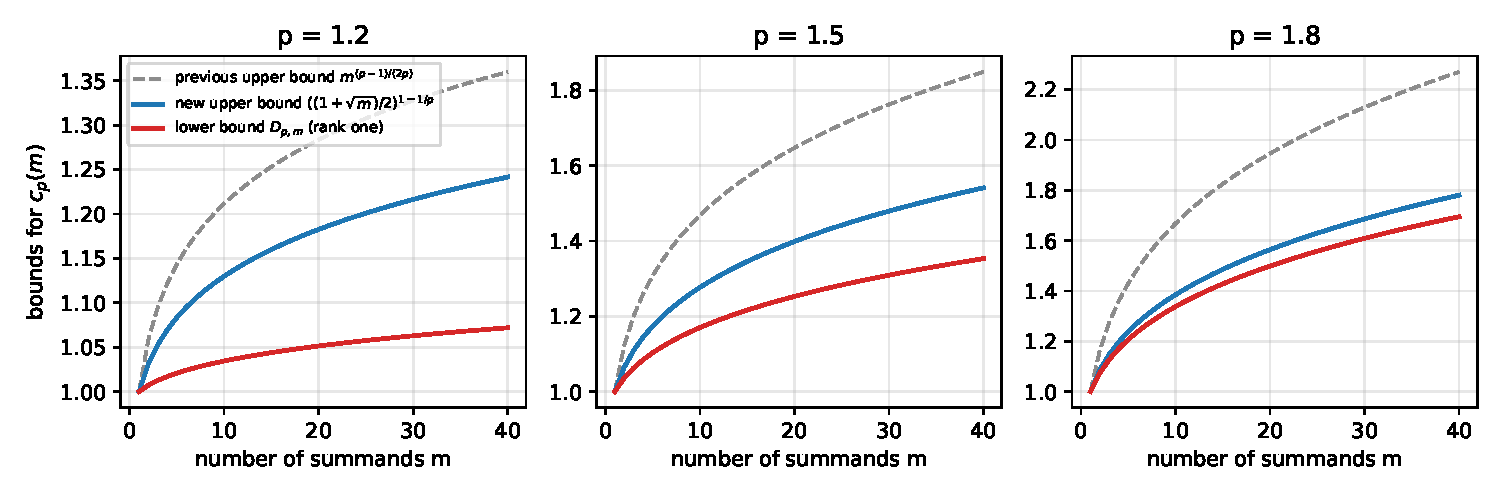
\includegraphics[width=\textwidth]{verification/bounds.pdf}
\caption{Bounds for the dimension-free constant \(c_p(m)\) as functions of
the number of summands \(m\), at \(p=1.2,1.5,1.8\): the rank-one lower
bound \(D_{p,m}\) (red), the interpolation bound of
Corollary~\ref{cor:interp} (blue) and the earlier bound \(m^{(p-1)/(2p)}\)
(dashed). The true constant lies between the red and blue curves.}
\label{fig:bounds}
\end{figure}

\begin{remark}[Two consistency checks]\label{rem:logconvex}
(i) Since \(c_p(n,n)=D_{p,n}\) for \(1<p<2\) and the endpoint values are
\(1\) and \(\sqrt{(1+\sqrt n)/2}\), Theorem~\ref{thm:interp} implies
that \(1/p\mapsto\log D_{p,n}\) is convex on \([1/2,1]\). This purely
scalar statement is confirmed numerically by the accompanying script for
\(n=2,3,5,10\). (ii) For \(p>2\), interpolating between \(p=2\) and
\(p=\infty\) gives a bound weaker than Qiu's exact value; the interpolation
bound is useful only below \(p=2\).
\end{remark}

\section{Beyond rank one: certified witnesses}\label{sec:beyond}

This section proves Proposition~\ref{prop:certified} and describes what
the numerics suggest about the gap between arbitrary and rank-one
summands when \(m<n\).

\paragraph{The witnesses.}
For each listed \(p\) the file \texttt{verification/witnesses.json} gives
rational \(3\times3\) data \(K_1,K_2\) (skew-symmetric) and \(C_1,C_2\).
Put \(O_k=(I-K_k)(I+K_k)^{-1}\), an orthogonal matrix with rational entries
(Cayley transform), \(H_k=C_k^TC_k\ge0\) and \(A_k=O_kH_k\). Then
\(|A_k|=H_k\) exactly, so the quotient in Proposition~\ref{prop:certified}
equals \(\bigl(\sum_i\lambda_i^{p/2}\bigr)^{1/p}/
\bigl(\sum_i\mu_i^p\bigr)^{1/p}\), where \(\lambda_i\) are the eigenvalues
of \(N^TN\), \(N=A_1+A_2\), and \(\mu_i\) those of \(H_1+H_2\). All of
these are roots of cubic polynomials with rational coefficients. The data
were found by numerical optimisation over this parametrisation and then
rounded to rationals.

\begin{proof}[Proof of Proposition~\ref{prop:certified}]
For each \(p\), the script \texttt{certify\_rank\_gap.py} computes
\(O_k,H_k,N\) in exact rational arithmetic, checks \(O_k^TO_k=I\),
isolates the eigenvalues of \(N^TN\) and of \(H_1+H_2\) in rational
intervals of width at most \(10^{-40}\) (exact real-root isolation), and
encloses the quotient with interval arithmetic. It encloses \(D_{p,2}\)
from above as follows: by Lemma~\ref{lem:scalar}, \(F_{p,2}\) increases up
to \(x_{p,2}\) and decreases after it; the script brackets \(x_{p,2}\) in a
rational interval on whose endpoints the left side of \eqref{eq:critical}
has certified opposite signs, and bounds \(F_{p,2}\) on that interval by
interval evaluation. In every case the lower end of the quotient
enclosure exceeds the upper bound for \(D_{p,2}\); Table~\ref{tab:cert}
lists the values (the displayed decimals are rounded outward from
60-digit values). The trusted base is exact rational arithmetic, sympy's
real-root isolation and mpmath's interval elementary functions. The script also checks that each quotient is below a
certified lower bound for \(D_{p,3}\), as Theorem~\ref{thm:main} requires.
Finally, embedding \(M_3\) in \(M_n\) shows that \(c_p(2,n)\) is
non-decreasing in \(n\), so \(c_p(2,n)\ge c_p(2,3)>D_{p,2}=c_p(2,2)\) for
\(n\ge3\), and \(c_p(2)>D_{p,2}\).
\end{proof}

\begin{table}[ht]
\centering
\small
\begin{tabular}{@{}lll@{}}
\toprule
\(p\) & certified quotient \(\ge\) & \(D_{p,2}\le\)\\
\midrule
\(11/10\) & 1.002012486 & 1.001997012\\
\(6/5\) & 1.007357637 & 1.007324966\\
\(5/4\) & 1.011023115 & 1.010987535\\
\(13/10\) & 1.015244511 & 1.015210078\\
\(4/3\) & 1.018334201 & 1.018302376\\
\(7/5\) & 1.025092913 & 1.025069071\\
\(3/2\) & 1.036425091 & 1.036414358\\
\(8/5\) & 1.048783502 & 1.048780904\\
\(17/10\) & 1.061667909 & 1.061667713\\
\bottomrule
\end{tabular}
\caption{Certified witnesses for \(c_p(2,3)>D_{p,2}\) (two real
\(3\times3\) summands with rational entries).}
\label{tab:cert}
\end{table}

\paragraph{What the numerics suggest.}
For \(m=2\), \(n=3\) the certified excess over \(D_{p,2}\) in
Table~\ref{tab:cert} is between \(1.5\times10^{-5}\) and
\(3.6\times10^{-5}\) for \(1.1\le p\le1.4\), about \(1.1\times10^{-5}\) at
\(p=3/2\), \(2.6\times10^{-6}\) at \(p=8/5\) and \(2\times10^{-7}\) at
\(p=17/10\). Numerical optimisation in the accompanying script finds an
excess of only about \(8\times10^{-10}\) at \(p=1.8\) and none detectable
at \(p=1.9\). At \(p=2\) there is no gap
\cite[Theorem 6.2]{Zhang}. The optimisers found are close to rank-one
families with a small second singular value in one summand. We do not know
whether the gap is positive for every \(p<2\), or whether rank-one families
are again optimal above some threshold \(p^*<2\).

\paragraph{A perturbative criterion (heuristic).}
A natural route to \(c_p(m,m+1)>D_{p,m}\) for every \(1<p<2\) is to perturb
a rank-one extremiser into one extra dimension. Giving a summand a second
singular value \(\sigma\) whose vectors leave the support of \(B\) changes
\(\|B\|_p^p\) and \(\|\sum A_k\|_p^p\) at order \(\sigma^p\) (the new
small eigenvalues), while the remaining changes are of order \(\sigma^2\).
Since \(p<2\), the sign of the first-order effect is decided by comparing
two order-\(\sigma^p\) coefficients, a one-direction quotient that must
exceed \(D_{p,m}\). Whether it does so for every \(p<2\) is open, and the
numerics above suggest that it may fail near \(p=2\)
(Section~\ref{sec:open}, item~3).

\section{A consequence for concave functions}\label{sec:concave}

This section records what Li's transfer theorem gives when combined with
Theorem~\ref{thm:main}. Li \cite[Theorem 1.1]{Li} proved that, for each
fixed \(p,m,n\), the best constant valid simultaneously for all
nonnegative concave \(f:[0,\infty)\to[0,\infty)\) in
\[
 \Bigl\|f\Bigl(\Bigl|\sum_kA_k\Bigr|\Bigr)\Bigr\|_p
 \le c\,\Bigl\|\sum_kf(|A_k|)\Bigr\|_p
\]
equals the linear constant \(c_p(m,n)\). This is an external theorem; the
linear results above do not depend on it.

\begin{corollary}[Consequence of Li's theorem]\label{cor:concave}
For \(m\ge n\), \(1<p<2\), \(A_k\in M_n(\C)\) and every nonnegative concave
\(f\) on \([0,\infty)\),
\begin{equation}\label{eq:concave}
 \Bigl\|f\Bigl(\Bigl|\sum_{k=1}^mA_k\Bigr|\Bigr)\Bigr\|_p
 \le D_{p,n}\Bigl\|\sum_{k=1}^mf(|A_k|)\Bigr\|_p .
\end{equation}
The constant is sharp for the whole class (already for \(f(t)=t\)) and
also for each cap function \(f(t)=\min(t,r)\), \(r>0\).
\end{corollary}

\begin{proof}
Combine Li's Theorem~1.1 with Theorem~\ref{thm:main}. For each fixed cap,
Li's Theorem~2.3 identifies its sharp constant with the linear one.
\end{proof}

We make no claim of individual sharpness for other fixed concave
functions; the corollary is a consequence of Li's theorem, not a new
transfer principle. Similarly, Theorem~\ref{thm:interp} and Li's theorem
together give the bound of Corollary~\ref{cor:interp} for the concave
problem.

\section{Open problems}\label{sec:open}

This section lists what remains open, with the best bounds known to us.
\begin{enumerate}
\item \emph{Lee's problem for \(1<p<2\).} Determine \(c_p(2)\). Known:
\(D_{p,2}<c_p(2)\le((1+\sqrt2)/2)^{1-1/p}\), with the strict lower
inequality certified at the nine exponents of
Proposition~\ref{prop:certified}; at \(p=3/2\),
\(1.0364250<c_{3/2}(2)<1.0647523\).
\item \emph{The dimension-free constant \(c_p(m)\).} Is the ratio
\(c_p(m)/m^{(p-1)/(2p)}\) convergent, and is its limit \(2^{-1/p}\) (the
rank-one value) or larger? Corollary~\ref{cor:interp} confines it to
\([2^{-1/p},2^{-(p-1)/p}]\) asymptotically.
\item \emph{Arbitrary rank with \(m<n\).} Determine \(c_p(m,n)\) for
\(m<n\). Known: \(\max\{D_{p,m},\ \text{certified witnesses}\}\le
c_p(m,n)\le\min\{D_{p,n},((1+\sqrt m)/2)^{1-1/p}\}\), the first upper
bound being strict. Is \(c_p(m,n)>D_{p,m}\) for every \(n>m\) and every
\(1<p<2\), or is there a threshold \(p^*<2\) above which rank-one families
are optimal? Does \(c_p(m,n)\) stabilise in \(n\)?
\item \emph{Why the method stops.} The factorisation \eqref{eq:factor}
sees only the spectrum of \(B=\sum|A_k|\), not how \(B\) is split into
\(m\) pieces. Any exact answer for \(m<n\) must use that splitting.
\end{enumerate}

\section*{Computations and AI use}
The proofs above are complete without computer assistance, except
Proposition~\ref{prop:certified}, which is a computer-assisted proof in
exact rational and interval arithmetic. The accompanying scripts are
\texttt{verification/certify\_rank\_gap.py} (the certificate, with its
data \texttt{verification/witnesses.json}),
\texttt{verification/verify\_schatten.py} (numerical checks of the
scalar constant, equality families, random and adversarially optimised
families, the radical, Qiu's example, the bounds of
Table~\ref{tab:bounds} and the asymptotics, with negative controls) and
\texttt{verification/plot\_bounds.py} (Figure~\ref{fig:bounds}). Apart
from the certificate, the numerical checks supplement and do not replace
the proofs. This paper was prepared with substantial assistance from AI
systems, which were used for drafting, proof development, literature
search and computation; the mathematical content was checked by
independent AI-assisted reviews and by the scripts above. It has not been
peer reviewed.

\begin{thebibliography}{99}

\bibitem{BourinZhang}
Bourin, J.-C., \& Zhang, T. (2026).
Matrix triangle inequalities: past, present, and future.
\emph{Reviews in Mathematical Physics}, S0129055X26500236.
\url{https://doi.org/10.1142/s0129055x26500236}
(arXiv:2610.30538).

\bibitem{Harremoes}
Harremoës, P. (2009).
Joint range of Rényi entropies.
\emph{Kybernetika, 45}(6), 901--911.
\url{https://www.kybernetika.cz/content/2009/6/901/paper.pdf}

\bibitem{Lee2010}
Lee, E.-Y. (2010).
Rotfel'd type inequalities for norms.
\emph{Linear Algebra and its Applications, 433}, 580--584.
\url{https://doi.org/10.1016/j.laa.2010.03.029}

\bibitem{Lee2012}
Lee, E.-Y. (2012).
How to compare the absolute values of operator sums and the sums of
absolute values?
\emph{Operators and Matrices, 6}(3), 613--619.
\url{https://doi.org/10.7153/oam-06-42}

\bibitem{Li}
Li, X. (2026).
\emph{Sharp concave-function transfer for Lee-type Schatten norm
inequalities} (arXiv:2608.25989v1). Preprint.
\url{https://arxiv.org/abs/2608.25989v1}

\bibitem{LinZhang}
Lin, J., \& Zhang, Y. (2022).
A proof of Lee's conjecture on the sum of absolute values of matrices.
\emph{Journal of Mathematical Analysis and Applications, 516}(2), 126542.
\url{https://doi.org/10.1016/j.jmaa.2022.126542}

\bibitem{Pang}
Pang, Z. (2026).
\emph{Counterexamples to a conjectured Schatten norm inequality}
(arXiv:2608.18112v1). Preprint.
\url{https://arxiv.org/abs/2608.18112v1}

\bibitem{Qiu}
Qiu, H. (2026).
\emph{Sharp quasi-reverse Minkowski inequality for Schatten norms}
(arXiv:2608.17565v2). Preprint.
\url{https://arxiv.org/abs/2608.17565v2}

\bibitem{SakaiIwata}
Sakai, Y., \& Iwata, K.-i. (2016).
\emph{Sharp bounds between two Rényi entropies of distinct positive
orders} (arXiv:1605.00019). Preprint.
\url{https://arxiv.org/abs/1605.00019}

\bibitem{Stein}
Stein, E. M. (1956).
Interpolation of linear operators.
\emph{Transactions of the American Mathematical Society, 83}(2), 482--492.
\url{https://doi.org/10.1090/S0002-9947-1956-0082586-0}

\bibitem{Thompson}
Thompson, R. C. (1976).
Convex and concave functions of singular values of matrix sums.
\emph{Pacific Journal of Mathematics, 66}(1), 285--290.
\url{https://doi.org/10.2140/pjm.1976.66.285}

\bibitem{TangZhang}
Tang, Q., \& Zhang, S. (2026).
Generalizing Lee's conjecture on the sum of absolute values of matrices.
\emph{Linear Algebra and its Applications, 731}, 196--204.
\url{https://doi.org/10.1016/j.laa.2025.11.015}
(arXiv:2510.16846).

\bibitem{Zeng}
Zeng, Z., Liu, H., \& Ratnavelu, K. (2026).
\emph{A counterexample to the Tang--Zhang Schatten norm conjecture and
sharp positive results} (arXiv:2608.15558). Preprint.
\url{https://arxiv.org/abs/2608.15558}

\bibitem{ZengInterval}
Zeng, Z., Liu, H., \& Ratnavelu, K. (2026).
\emph{The Tang--Zhang Schatten norm formula fails below the Hilbertian
exponent}. Manuscript SM1-P01, AI-Has-Taste archive.
\url{https://github.com/ArtificialZeng/AI-Has-Taste/blob/main/pdfs/smallmac_1/SM1-P01_Tang_Zhang_Schatten_Norm_Formula.pdf}

\bibitem{ZengExact}
Zeng, Z., Liu, H., \& Ratnavelu, K. (2026).
\emph{The exact Schatten 3/2 constant for two rank-one matrices}.
Manuscript SM1-P02, AI-Has-Taste archive, commit
\texttt{2537a78914f784a42b3f6ff3677d93ba0f31e97e} (13 September 2026).
\url{https://github.com/ArtificialZeng/AI-Has-Taste/blob/main/pdfs/smallmac_1/SM1-P02_Exact_Schatten_Three_Halves_Constant.pdf}

\bibitem{Zhang}
Zhang, T. (2026).
Operator symmetric moduli and sharp triangle inequalities.
\emph{Journal of the London Mathematical Society, 114}(2), e70672.
\url{https://doi.org/10.1112/jlms.70672}
(arXiv:2603.01046; theorem numbers refer to arXiv v1).

\end{thebibliography}
\end{document}
